\documentclass{article}
\usepackage[utf8]{inputenc}

\title{IF796 - Mineração da Web}
\author{Carlos Augusto Mendes Valença}
\date{03 de Maio de 2019}

\usepackage{natbib}
\usepackage{graphicx}

\begin{document}

\maketitle

\section{Introdução}
A Mineração da Web é uma disciplina da área de Recuperação de Informação (RI) que trabalha com obtenção e organização de informações, documentos e outras formas de organização de dados, assim como trabalhar com bases de índices. 

\section{Relevância}
A disciplina é importante graças à sua aplicação em diversas áreas da Computação relacionadas à manejo de informações, como, por exemplo sistemas da Web como engenhos de busca e sistemas de recomendações a usuários, a exemplo do sistema do Youtube, assim como ferramentas do tipo Page Rank. Portanto, tem muita utilidade em sistemas de empresas, podendo fazer a comunicação empresa-usuário.

\begin{figure}[h!]
\centering
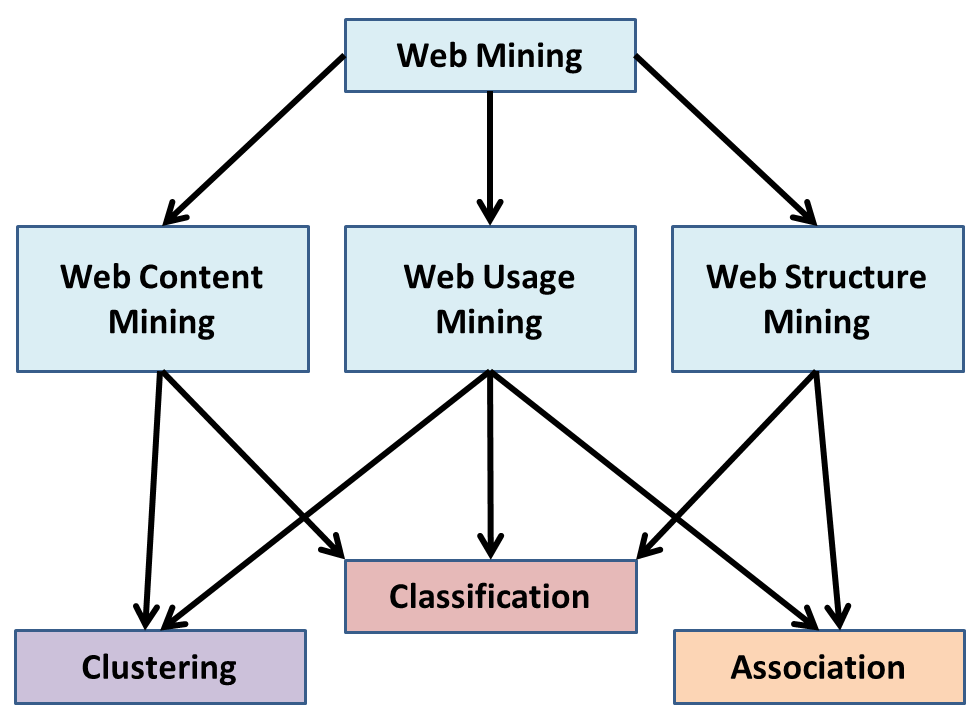
\includegraphics[scale=0.4]{web_mining}
\caption{Fluxograma da Mineração da Web e algumas de suas subdivisões.}
\label{fig:web_mining}
\end{figure}

\section{Relação com outras disciplinas}
\begin{table}[]
\begin{tabular}{ll}
IF684 - Sistemas Inteligentes                                                         & \begin{tabular}[c]{@{}l@{}}A disciplina de Sistemas Inteligentes é \\ importante porque ela trabalha justamente\\ com aprendizagem a partir de dados, ou seja,\\ os Sistemas Inteligentes estão diretamente\\ relacionados à Mineração da Web no tocante  \\ aos métodos como os dados são usados.\end{tabular}                                    \\
\begin{tabular}[c]{@{}l@{}}IF685 - Gerenciamento de Dados\\ e Informação\end{tabular} & \begin{tabular}[c]{@{}l@{}}A disciplina de Gerenciamento de Dados também\\ se relaciona com a de Mineração da Web através\\ do método como os dados sobre determinado assunto\\ são obtidos e utilizados.\end{tabular}
\end{tabular}
\end{table}

\pagebreak

\section{Conclusão}
A partir do informado, é visível a importância da Mineração da Web e da Recuperação de Informação, pois permitem maior participação do usuário nos processos desenvolvidos no espaço digital. Sendo assim, a disciplina é importante para muitas coisas relacionadas ao manejo e manipulação de dados na Web.    

\citep{baezayates2010mir}
\citep{introductionir}
\citep{slidesif796}

\bibliographystyle{plain}
\bibliography{camv}
\end{document}
